\chapter{RESULTADOS E DISCUSSÕES}

O protótipo funcional resultado da aplicação desta pesquisa é ilustrado na
\autoref{transmission-at-gnome}, e evidencia as adaptações propostas na
interface do Transmission.

Foi utilizada a mesma transição observada na interface do Evince, onde a barra
de títulos é substituída por uma 

A barra de título foi substituida por uma \textit{Header Bar}, agregando parte
dos botões antes presentes na \textit{Toolbar}

\begin{figure}[!h]
  \begin{center}
    \caption{\textbf{Transmission no GNOME 3.16}}
    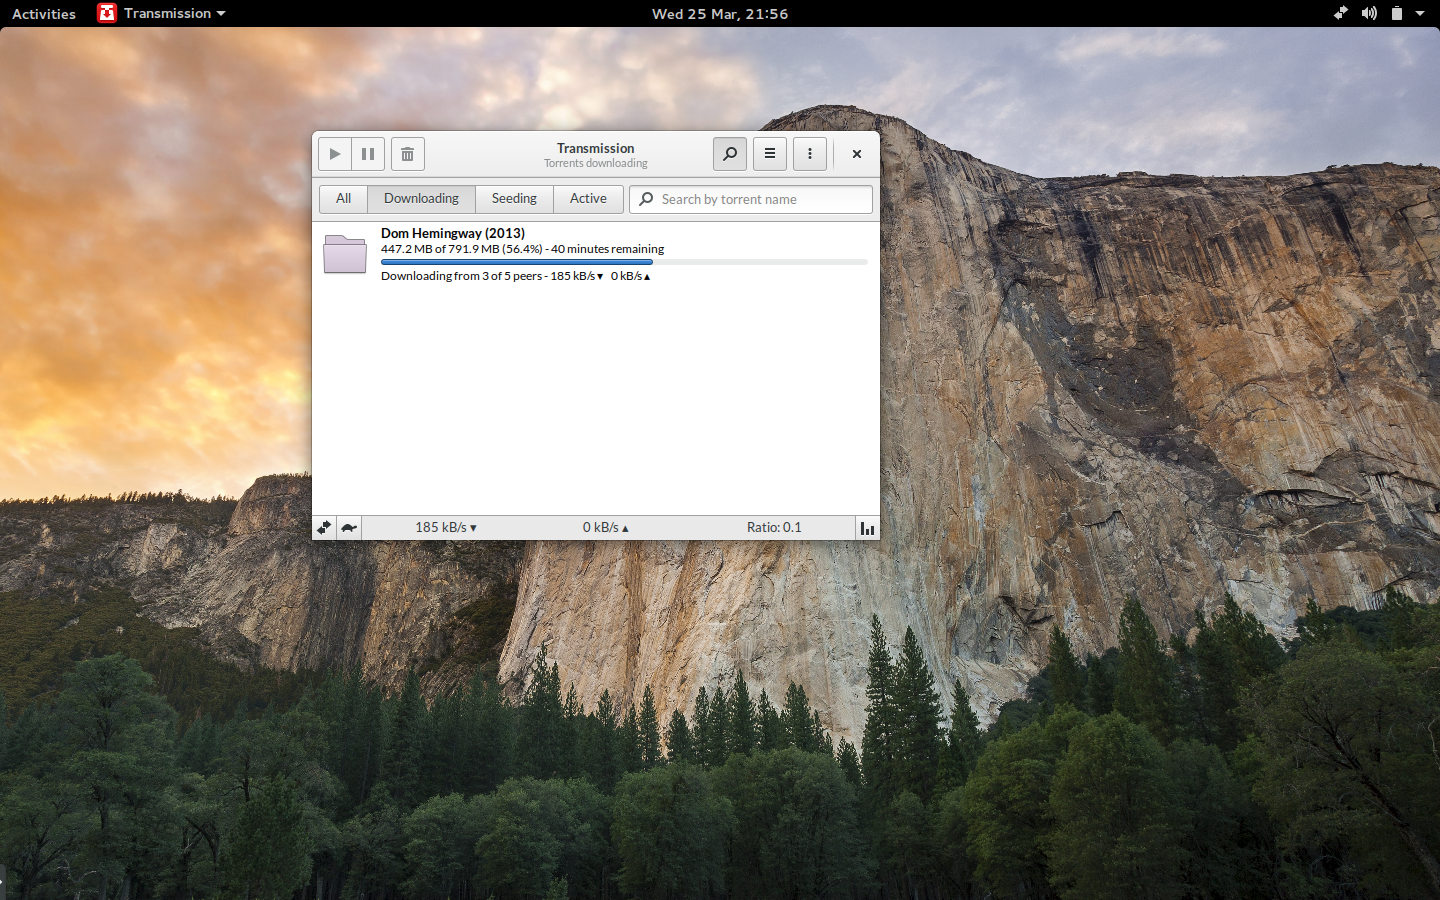
\includegraphics [scale=0.2]{image/transmission-gtk3-main.png}
    \label{transmission-at-gnome}
  \end{center}
\end{figure}

\section{A evolução das aplicações centrais analisadas}

Percebeu-se uma tendencia de redução da razão área útil vs controles em todas
aplicações centrais. A \autoref{workarea-vs-chrome} apresenta a razão
coletada em cada aplicação e versão:

\begin{table}[htb]
\ibgetab{
  \caption{Área útil vs Controles}
  \label{workarea-vs-chrome}
}{
    \begin{tabular}{ | l | l | l | } 
    \hline
    Aplicação & Versão 3.6 & Versão 3.16 \\ \hline
    Nautilus  & 171 pixels & 171 pixels \\
    Evince    & 116 pixels & 171 pixels \\
    Gedit     & 70 pixels  & 171 pixels \\
    \hline
    \end{tabular}
}{
  \fonte{Do Autor}
}
\end{table}

Tal tendência se repete na remodelagem da forma e função de vários widgets, uma
clara influência de ambos design de usabilidade e da redução de espaço vertical,
visto a padronização de resoluções baseados na razão 16:9 (720p, 1080p, etc).

\subsection{Percepções do processo de transição}

Um dos elementos de interface mais comuns de um ambiente gráfico baseado em
janelas é a barra de título, por onde o usuário pode mover a janela no espaço de
trabalho. Até então, no GNOME, desenvolvedores tinham pouco ou nenhum controle
sobre elas por questões de compatibilidade de software.

No conceito de `Header Bars' as barras de título passam a poder acomodar botões,
caixas de texto, sliders, etc, substituindo as barras de ferramentas, antes
encontradas comumente abaixo de menus ou das barras de título, conforme a
\autoref{toolbar-positioning}.

\begin{figure}[!h]
  \begin{center}
    \caption{\textbf{Barra de Ferramentas no Evince e Gedit 3.6}}
    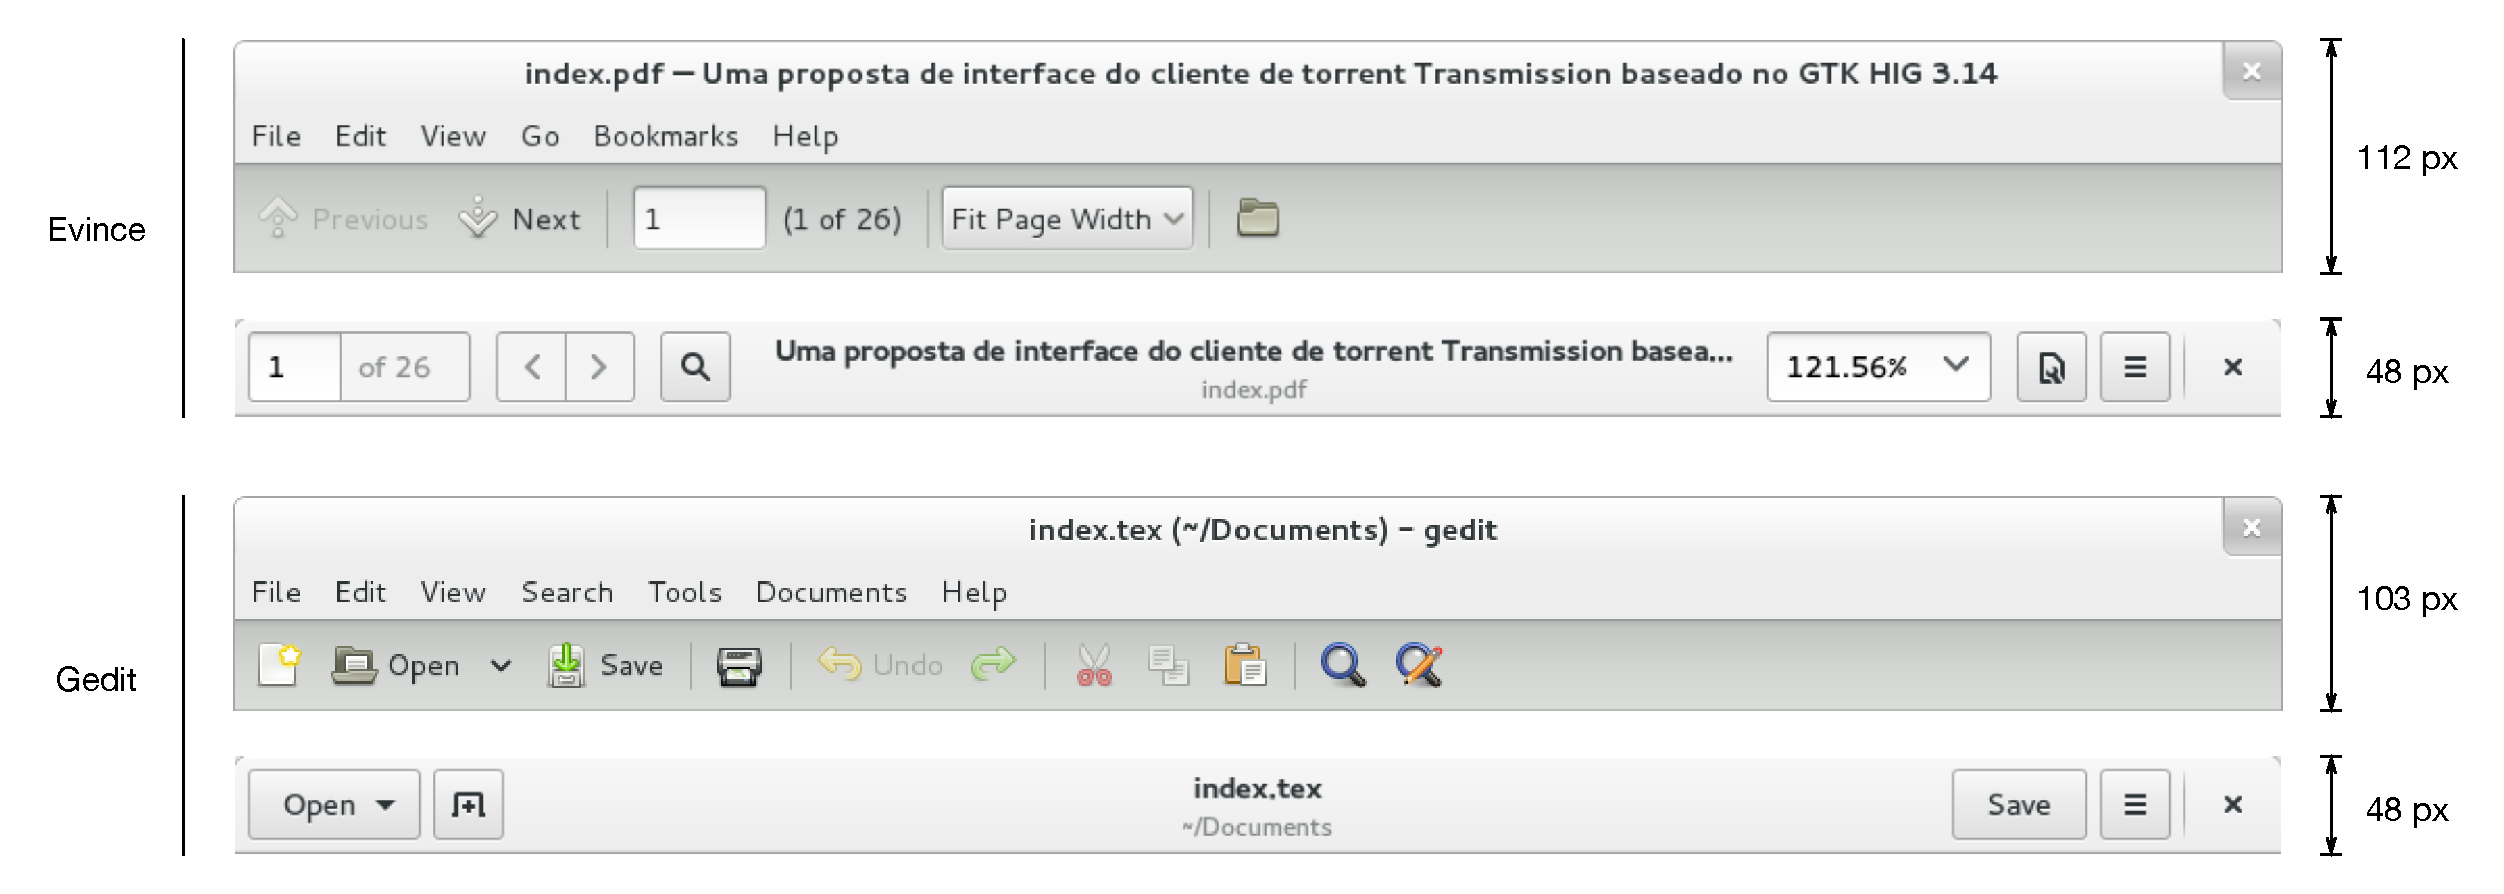
\includegraphics [width=\textwidth]{image/toolbar-headerbar-comparison.eps}
    \fonte{Do Autor}
    \label{toolbar-positioning}
  \end{center}
\end{figure}

Outra mudança notável foi a transição da barra de menus, quais ações foram
dissolvidas através de um ou mais widgets na janela do programa (sendo grande
maioria na Header Bar), nas ações pertinentes a janela, e em um menu de
aplicação, para ações pertinentes ao programa (Abrir, Sobre, Sair). A 
\autoref {rip-menubar} apresenta um mapeamento aproximado das ações da barra de
menus do Evince 3.6 para o 3.16.

\begin{figure}[!h]
  \begin{center}
    \caption{\textbf{Mapeamento de menu no Evince}}
    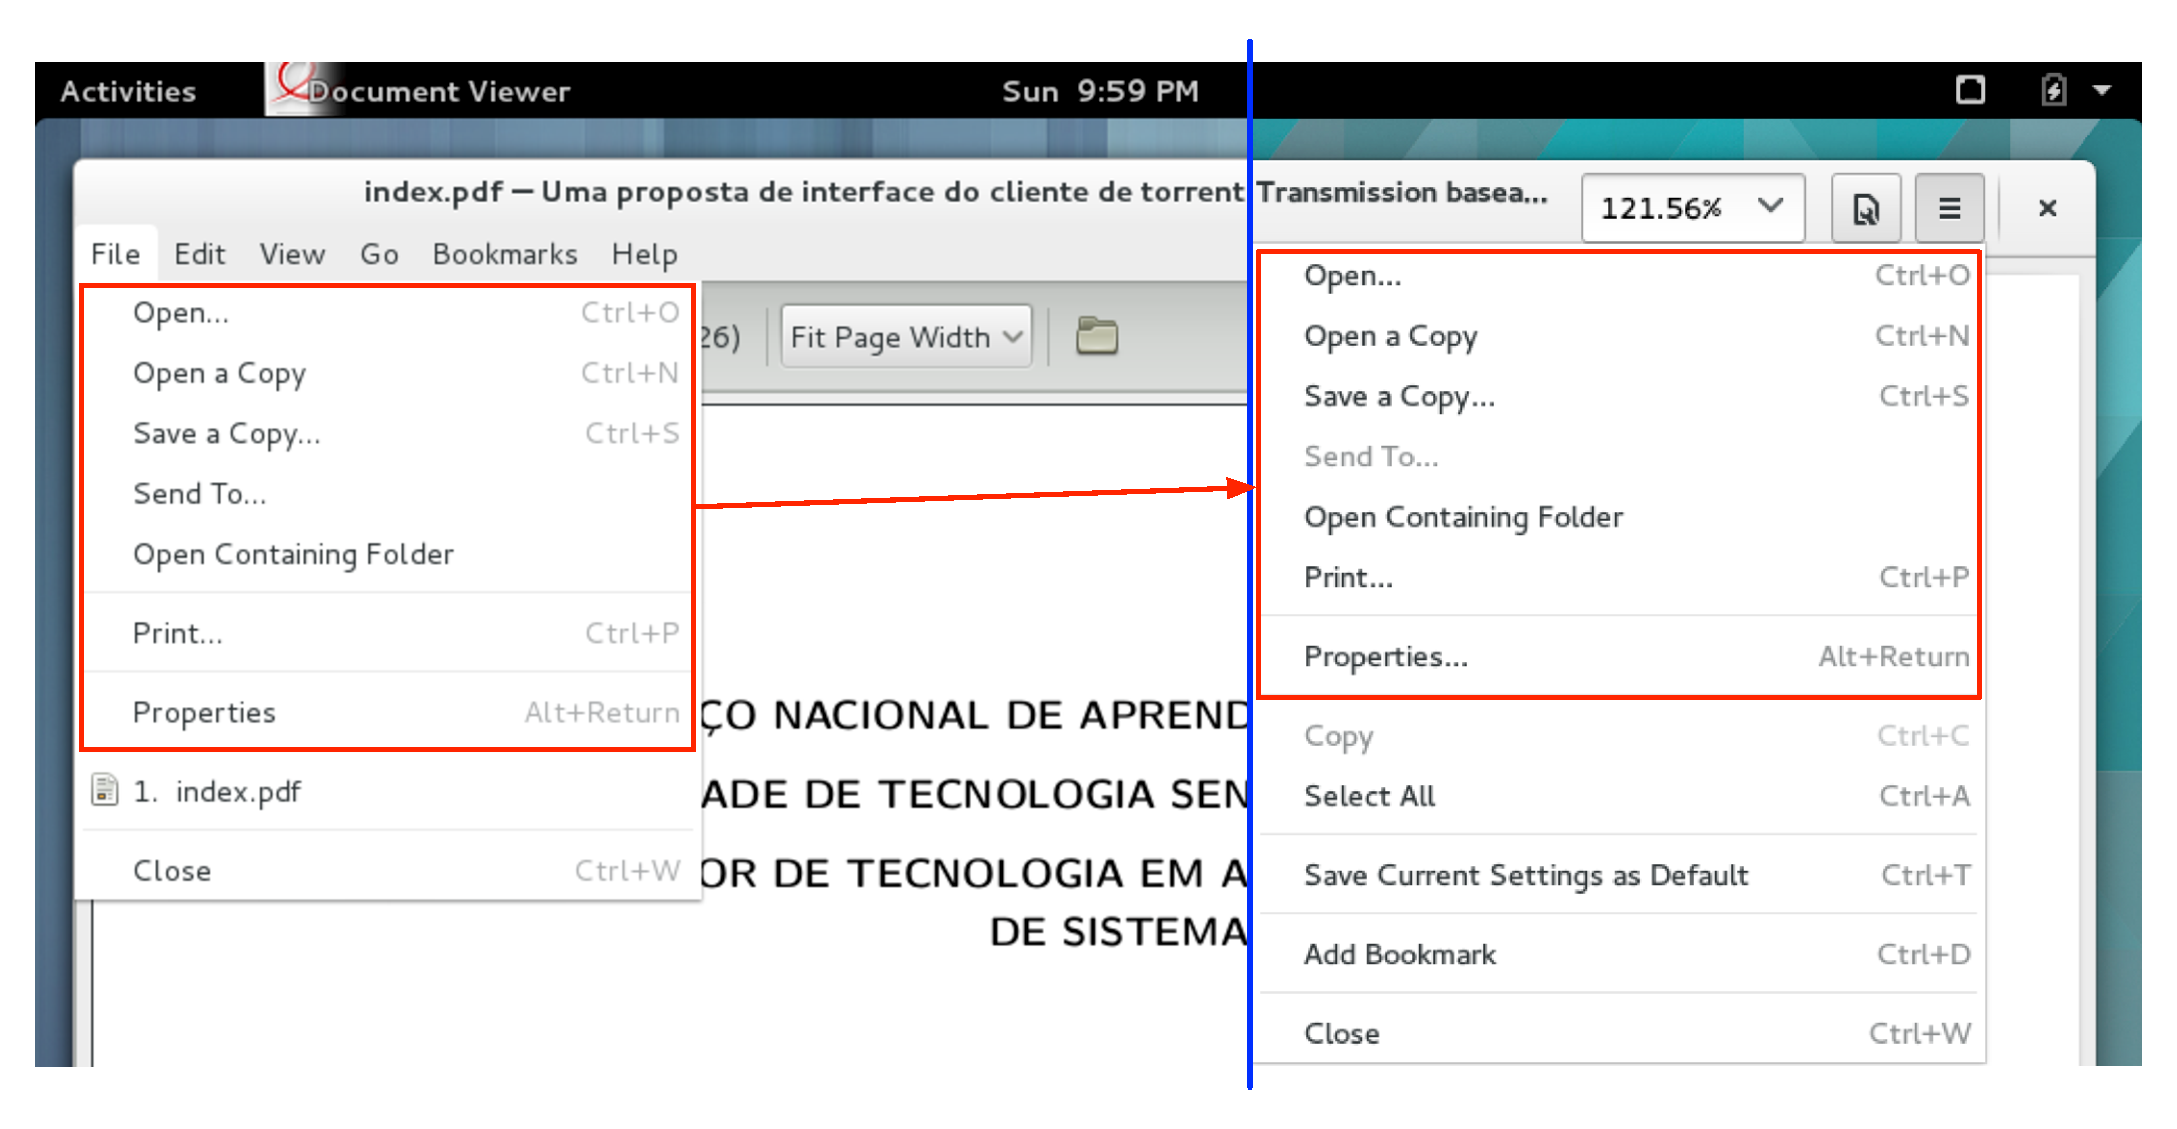
\includegraphics [width=\textwidth]{image/evince-menubar-mapping.eps}
    \label{rip-menubar}
  \end{center}
\end{figure}

A utilização do \textit{Revealer} em ambos \textit{Nautilus} e \textit{Evince}
também demonstrou-se eficaz como técnica para redução de espaço vertical e
aumento da área útil de ambos programas, através da exibição transiente da caixa
de busca, alternável pelo botão lupa no \textit{Header Bar}.

O \textit{Popover}, um elemento de interface introduzido no HIG 3.12, é uma
visão transiente e flutuante que permitite adicionar menus, listas e widgets
variados em seu interior, e é comumente usado como parte de menus ou menus de
contexto. Sua utilização foi observada em diversos pontos, inclusive como
coadjuvante na transição da barra de menus em todas aplicações analisadas.



\section{Header Bar}

A implementação da Header Bar no Transmission foi efetivada através da
dissolução das ações encontradas em ambas barra de ferramentas e menus em
botões. As ações da barra de menus foram separadas em duas categorias de menu:
Ações pertinentes ao programa e ações pertinentes a transferência selecionada,
posicionados da direita para a esquerda, respectivamente, conforme indicado pelo
HIG.

A \autoref{header-bar-transition} apresenta um paralelo entre a interface antiga
e a interface proposta, relacionando através de marcação em cores as transições
efetuadas. Os botões sensíveis a selecão (Iniciar, Parar e Remover) puderam ser
mantidos com seu comportamento original.

\begin{figure}[!ht]
  \begin{center}
    \caption{\textbf{Transição da Header Bar}}
    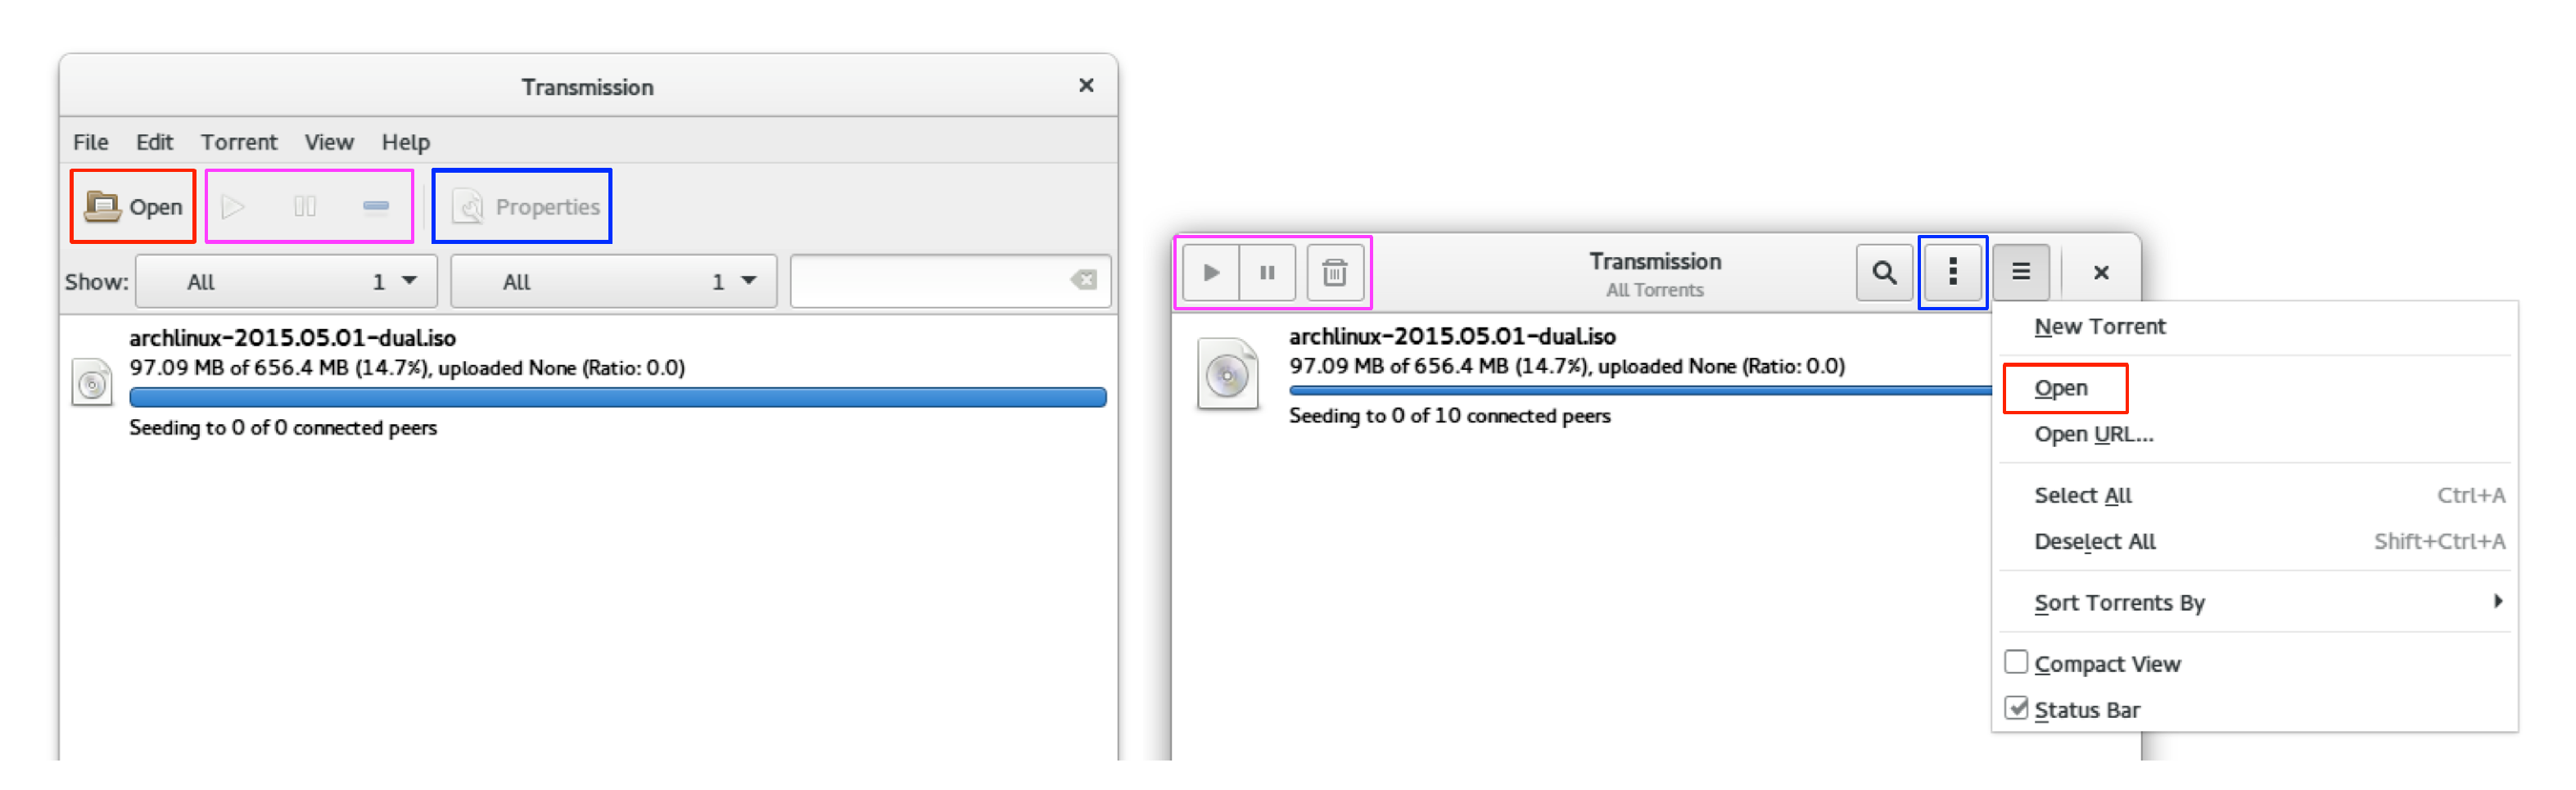
\includegraphics [width=\textwidth]{image/header-bar-transition.eps}
    \label{header-bar-transition}
    \fonte{Do Autor}
  \end{center}
\end{figure}

Pela natureza compacta da janela do Transmission e pelo compartilhamento do
espaço disponível na Header Bar pelos botões de ação e título da aplicação, a
adição excessiva de botões pode suprimir o título da janela, e a presença de um
número diferente de botões no lados direito e esquerdo pode fazer parecer com
que o título não esteja centralizado, causando desconforto visual. Por este
motivo os botões ``Properties'' e ``Open'' foram migrados para os menus, sendo
este movido para o menu de janela e aquele para o menu de seleção.

\section{Barra de Filtros}

Seguindo a implementação utilizada no Evince e Nautilus, os filtros de atividade
foram movidos juntamente a caixa de busca textual para um \textit{Revealer},
ativado através do botão com ícone de lupa, destacado na \autoref{revealer}.

\begin{figure}[!h]
  \begin{center}
    \caption{\textbf{Filtros retráteis através do uso de um Revealer}}
    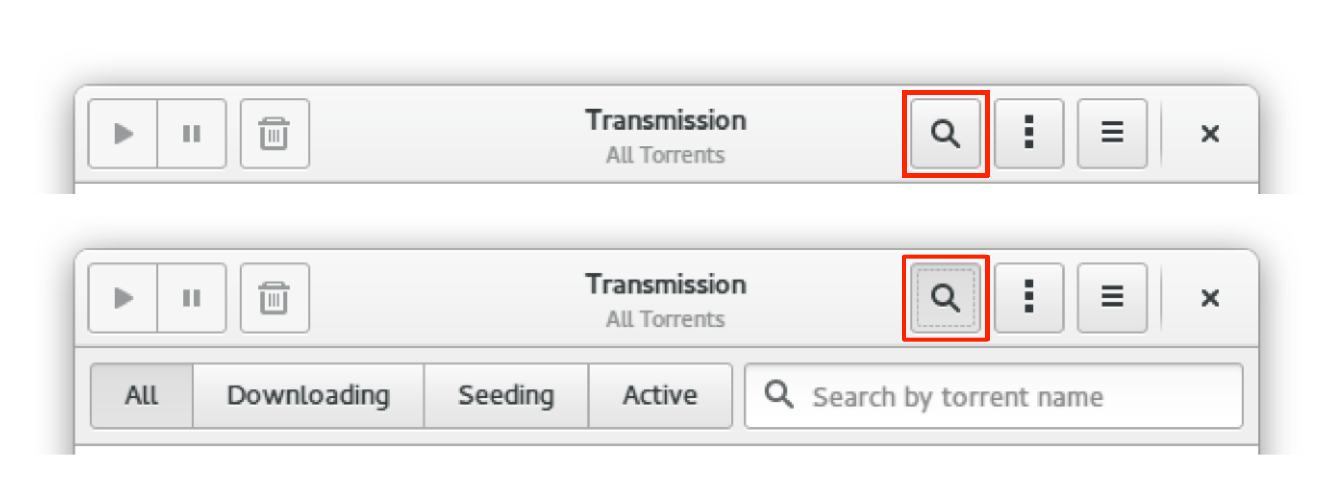
\includegraphics [width=\textwidth]{image/revealer.eps}
    \label{revealer}
    \fonte{Do Autor}
  \end{center}
\end{figure}

Na versão original do Transmission, além do filtro textual, existem dois tipos
de filtros adicionais: Por estado (Recebendo, Transmitindo, Parado) e por
\textit{tracker} (Servidores que auxiliam a troca de arquivos). Por questões de
poupança de espaço a funcionalidade de filtragem por \textit{tracker} foi
deliberadamente removida.

\section{Limites Globais de Upload/Download}

Utilizando-se de um padrão de design já existente na interface gráfica do
Transmission para Apple Mac OS X como fonte de inspiração, foi implementada a
configuração de limite de velocidade global utilizando um Popover, substituindo
o extenso menu existente anteriormente, de forma a permitir uma configuração
fácil e rápida com poucos cliques. A \autoref{global-limits-transition}
apresenta um paralelo entre a implementação original, a fonte de inspiração e o
resultado derivado.

\begin{figure}[!h]
  \begin{center}
    \caption{\textbf{Transição do menu de limites globais}}
    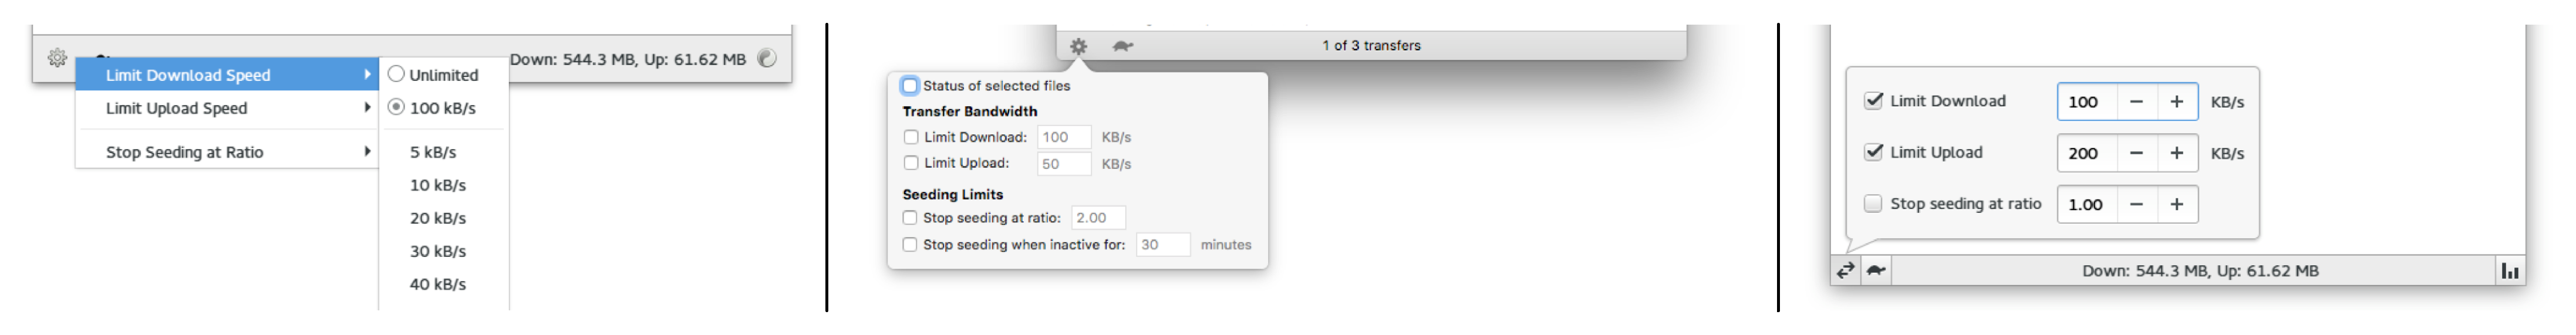
\includegraphics [width=\textwidth]{image/global-limits-transition.eps}
    \label{global-limits-transition}
    \fonte{Do Autor}
  \end{center}
\end{figure}

\section{Barra de Estado}

Todos os botões da barra de estado foram implementados utilizando ícones
simbólicos monocromáticos, de forma a se adaptarem a temas claros e escuros.
Também foi utilizado um Popover para implementar as opções de visualização das
estatísticas da barra de estado, funcionalidades ilustradas na 
\autoref{status-bar}.

\begin{figure}[!h]
  \begin{center}
    \caption{\textbf{Ícones simbólicos na barra de estado em temas claros e escuros}}
    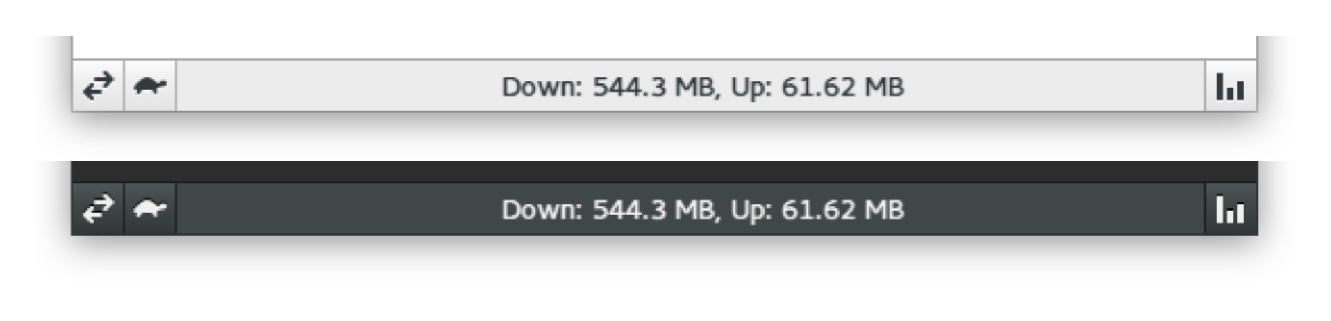
\includegraphics [width=\textwidth]{image/status-bar.eps}
    \label{status-bar}
    \fonte{Do Autor}
  \end{center}
\end{figure}
